\chapter{The Boolean Satisfiability Problem}\label{chap:preliminaries}
\minitoc
In this thesis, our goal is to exploit the symmetrical properties of SAT problems.
Before, we get to the heart of the matter, we first introduce the Boolean satisfiability (SAT)  problem.
This problem is a propositional formula representing the constraints of a system.
A tool that aims to satisfy such formulas is called a SAT solver. 

%It answers $\sat$ when all constraints
%present in the formula can be satisfied and $\unsat$ otherwise.


\section{SAT basics}
The satisfiability problem is constituted of \emph{Boolean} or \emph{propositional variable}.
It has two possible values, true or false (noted respectively $\true$ or $\false$).
We call \emph{literal}, a propositional variable or its negation.
For a given variable $x$, the positive literal is represented by $x$ and the negative one by $\neg x$.
Given a formula $\varphi$, we denote $\Vars_\varphi$ ($\Lits_\varphi$) the set of variables (literals) used in the formula (the index in $\Vars_\varphi$ and $\Lits_\varphi$ is usually omitted when
clear from context).
To build more complex formula, it exists different operators, $\neg, \lor$ and $\land$ that are respectively negation, disjunction and conjunction. Others operators like $\Rightarrow, \Leftrightarrow$ and
$\oplus, \cdots$ respectively called implication, equivalence and exclusive disjunction (xor), $\cdots$ can be 
expressed with the basic ones.
For example $a \Rightarrow b$ can be expressed as $ \neg a \lor b$.
To ensure the priority of these operators, constraints are expressed between parenthesis.
In the absence of its, the following priority order applies (from the highest to the lowest priority):
negation ($\neg$), conjunction ($\land$), disjunction ($\lor$).


The value given to each variable of a formula is called an \emph{assignment} noted $\alpha$ and defined as follows:
 $$\alpha: \Vars \mapsto \{ \true, \false \}$$
 As usual $\alpha$ is said \emph{total}, or \emph{complete}, when all elements of $\Vars$ have an image by
$\alpha$, otherwise it is \emph{partial}. By abuse of notation, an assignment is
often represented by the set of its true literals. For example, $\alpha = \{\neg x_1, x_3 \}$ means that $x_1$
have the false value and $x_3$ have the true value.
  The set of all (possibly partial) assignments of $\Vars$ is noted $\Assignments(\Vars)$.
A \emph{truth table} gives an evaluation of all possible assignments for a given formula.
\Cref{tab:truthtable} shows the evaluation of negation ($\neg$), conjunction ($\land$), disjunction ($\lor$) operators.
For convenience, true value (\true) is also represented by $1$ and false value (\false) is represented by $0$.
When a formula is always true independently from the assignment, it is called a \emph{tautology} $x \lor \neg x$ is 
an example of tautologous formula.


\begin{table}[!htbp]
	\centering
	\begin{tabular}{cc|ccc}
		$x$ & $y$ & $\neg x$ & $x \lor y$ & $x \land y$ \\
		\toprule
		0 & 0 & 1 & 0 & 0 \\
		\midrule
		0 & 1 & 1 & 1 & 0 \\
		\midrule
		1 & 0 & 0 & 1 & 0 \\
		\midrule
		1 & 1 & 0 & 1 & 1 \\
		\bottomrule
	\end{tabular}
	\caption{Truth table of basic operators}
	\label{tab:truthtable}
\end{table}

\subsection{Normal forms}
In Boolean logic, it exists some structural properties, called \emph{normal form}.
To present them, we first need to introduce \emph{clause} and \emph{cube} concepts.
A \emph{clause} $\omega$ is a finite disjunction of literals:
$$\omega = \bigvee_{i=1}^k l_i \text{ , or the set of its literals } \omega = \{l_i\}_{i \in \llbracket 1,k \rrbracket}$$
 
A \emph{cube} $\gamma$ is a finite conjunction of literals represented by:
$$\gamma = \bigwedge_{i=1}^k l_i$$

% Or equivalently by the set of its literals:
%$$\omega = \{l_i\}_{i \in \llbracket 1,k \rrbracket}$$
With respect to its size, a clause is said to be \emph{unary, binary, ternary, $n$-ary} if it contains respectively one, two, three, or $n$ literals.

The clause form has a property called \emph{subsumption}. 
When a clause $\omega_1$ is a subset of another clause $\omega_2$ noted $\omega_1 \subset \omega_2$. And any 
assignment that satisfies $\omega_1$ also satisfies $\omega_2$, so $\omega_2$ is \emph{redundant} towards $\omega_1$ and so can be removed of the formula.

\emph{Conjunctive Normal Form} (CNF) of a formula is a finite conjunction of clauses:
  $$\varphi = \bigwedge_{i=1}^k \omega_i$$
  
\emph{Disjunctive normal form} (DNF) of a formula is finite disjunction of cubes:
  $$\varphi = \bigvee_{i=1}^k \gamma_i$$
The following table is a summary of laws about Boolean formulas that allow to transform any formula to
a normal form.
\begin{table}[!htbp]
 \centering
 \begin{tabular}{lllc}
  
  \emph{associativity of $\lor$} & $(x \lor y) \lor z \equiv x \lor (y \lor z)$\\
  \emph{commutativity of $\lor$} & $x \lor y \equiv y \lor x$\\
  \emph{identity} & $x \lor \false \equiv x$\\
  \emph{domination} & $x \lor \true \equiv \true$\\
  \emph{idempotent} & $x \lor x \equiv x$\\
  \emph{distribution over $\land$} & $x \lor (y \land z) \equiv (x \lor y) \land (x \lor z)$\\
  
  \\
  \emph{associativity of $\land$} & $(x \land y) \land z \equiv x \land (y \land z)$\\
  \emph{commutativity of $\land$} & $x \land y \equiv y \land x$\\
  \emph{identity} & $x \land \true \equiv x$\\
  \emph{domination} & $x \land \false \equiv \false$\\
  \emph{idempotent} & $x \land x \equiv x$\\
  \emph{distribution over $\lor$} & $x \land (y \lor z) \equiv (x \land y) \lor (x \land z)$\\
   \\
   \emph{negation 1} & $x \lor \neg x \equiv \false$\\
    \emph{negation 2} & $x \land \neg x \equiv \true$\\
    
    \emph{double negation} & $\neg (\neg x) \equiv x$ \\
    \emph{De Morgan 1} & $\neg x \lor \neg y \equiv \neg (x \land y)$\\
    \emph{De Morgan 2} & $\neg x \land \neg y \equiv \neg (x \lor y)$\\
    
 \end{tabular}
 \caption{Set of laws of operators}
 \label{tab:laws}
\end{table}

Every formula can be transformed into a normal form with different complexity and the resulting formula is 
\emph{equivalent}.  
In other words, every assignment $\alpha$ that satisfies formula $\varphi$  also models the resulting formula $\psi$
and vice-versa, denoted by $\varphi \equiv \psi$.
 Also, we say a formula $\psi$ is a \emph{logical consequence} of a formula $\varphi$ is every model of $\varphi$
 is also a model of $\psi$ and is denoted by $\varphi \models \psi$.

Conjunctive normal form is the input form of state-of-the-art solvers. Any propositional
formula can be transformed in CNF form with a polynomial complexity. Conversely, DNF form have
an exponential memory complexity during the transformation.
Note that each cube in the problem in DNF form is a solution in the equivalent CNF formulas.
\hakan{Sharp SAT = transform CNF to DNF}

%A formula is said to be \emph{satisfiable} (\sat) if there is at least one assignment that satisfies it;
%otherwise the formula is \emph{unsatisfiable} (\unsat).

%\subsection{Satisfiability problem}
%A \emph{Boolean variable}, or \emph{propositional variable}, is a variable that
%has two possible values : true or false (noted respectively $\true$ or $\false$).
%A \emph{literal} $l$ is a propositional variable or its
%negation. For a given variable $x$, the positive literal is represented by $x$
%and the negative one by $\neg x$.
%
%A \emph{clause} $\omega$ is a finite disjunction of literals represented
%equivalently by $\omega = \bigvee_{i=1}^k l_i$ or the set of its literals
%$\omega = \{l_i\}_{i \in \llbracket 1,k \rrbracket}$. A clause with a single
%literal is called \emph{unit clause}.
%A clause is a \emph{tautology} if it is always true, a clause that contains a positive 
%and negative value of a clause for example.
%A \emph{conjunctive normal form (CNF) formula} $\varphi$ is a finite
%conjunction of clauses.  A CNF can be either noted $\varphi = \bigwedge_{i=1}^k
%\omega_i$ or $\varphi = \{\omega_i\}_{i \in \llbracket 1,k \rrbracket}$. We
%denote $\Vars_\varphi$ ($\Lits_\varphi$) the set of variables (literals) used in
%$\varphi$ (the index in $\Vars_\varphi$ and $\Lits_\varphi$ is usually omitted when
%clear from context).
%For a given formula $\varphi$, an \emph{assignment} of the variables of
%$\varphi$ is a function $\alpha: \Vars \mapsto \{ \true, \false \}$.  As usual, $\alpha$ is
%\emph{total}, or \emph{complete}, when all elements of $\Vars$ have an image by
%$\alpha$, otherwise it is \emph{partial}. By abuse of notation, an assignment is
%often represented by the set of its true literals.  The set of all (possibly
%partial) assignments of $\Vars$ is noted $\Assignments(\Vars)$.
%The assignment $\alpha$ \emph{satisfies} the clause $\omega$, denoted $\alpha
%\models \omega$, if $\alpha \cap \omega \neq \emptyset$. Similarly, the assignment
%$\alpha$ satisfies the propositional formula $\varphi$, denoted $\alpha \models
%\varphi$, if $\alpha$ satisfies all the clauses of $\varphi$. Note that a
%formula may be satisfied by a partial assignment. In this case, unassigned variable is called
%\emph{don’t care}.
%A formula is said to be
%\emph{satisfiable} (\sat) if there is at least one assignment that satisfies it;
%otherwise the formula is \emph{unsatisfiable} (\unsat).

\subsection{An NP-complete problem}
The SAT problem is the first NP-complete algorithm proven by Stephen Cook in 1971~\cite{cook1971complexity}.
NP-completeness means that a SAT problem can be solved with a non-deterministic Turing machine in polynomial time (NP) and is also NP-hard. A problem is said NP-hard if everything in NP can be transformed into it in polynomial time. 
One of the most important unsolved problems in theoretical computer science is the P versus NP problem.
This question is one of the seven millennium prize problems.


\subsection{Particular forms easy to solve}
In some particular forms, SAT problems can be computed with polynomial algorithm.


\textbf{2-SAT~\cite{aspvall1979linear}.}l
In this particular form, the given CNF formula contains only binary clauses.
In this case, it suffices to create a graph in which each clause is transformed into implication. For example, the clause $x \lor y$ will be transformed into $ \neg x \Rightarrow y,
\neg y \Rightarrow x$. After computing \emph{strong connected component} on this graph, to be looking for
 the positive and negative forms of the same variable, in the same  strong connected component suffices 
to determine the satisfiability of the formula. If it is the case, the formula is \unsat. Otherwise 
a solution can be deduce and the problem is \sat. This algorithm can be computed in linear time complexity.

\textbf{Horn SAT.} In this particular form, the given CNF formula contains only Horn clauses. It exists three form
of Horn clause: \emph{strict Horn clause} that contains only one positive literal and at least one negative literal,
\emph{positive Horn clause} that contains only one positive literal and no negative literals
\emph{negative Horn clause} that contains only negative literals.
To solve this particular form of formula, it suffices to  apply \emph{Boolean constraint propagation} (BCP) or \emph{unit propagation} explained thereafter in \cref{sec:dpll} until fix point.
Roughly speaking, It satisfies all unit clauses in cascade. Either an empty clause was deduced and the problem
is \unsat or the fix point is reached and the formula is \sat. Like 2-SAT, this algorithm can also be computed
in linear time complexity.


\textbf{XOR SAT.} In this particular form, each clause contains xor ($\oplus$) operator rather than or ($\lor$).
This problem can be seen as a system of linear equations. Gaussian elimination allows to solve this kind of
problem is polynomial time.

The membership of polynomial class (P) of the particular form of satisfiability problems describes above is a special case of Schaefer's dichotomy theorem~\cite{schaefer1978complexity}.

\subsection{Some related problems}

Different kind of problems related to SAT is presented is this section.
One of them is sharp-SAT (\#SAT), its purpose is to count the number of solutions in a CNF.


Another related problem is maximum satisfiability problem (MAX-SAT). In this case, the problem
is to find the maximum subset of clauses that can be satisfied for a formula. Different variants
of this problem exist. For example, some constraints must be satisfied (hard clauses) and MAX-SAT
is applied on the remaining clauses called \emph{soft} clauses.

The last related problem is quantified Boolean formula (QBF) where the quantifiers $\exists$ and
$\forall$ are present in the formula. For example, $\forall x\, \exists y\, \exists z \, (x \lor y) \land z$.
This particular form is a generalization of the SAT problem with PSPACE complexity.

\subsection{Solving a SAT problem}
Two kinds of algorithms exist to solve satisfiability problems.
First, the \emph{incomplete} algorithm~\cite{biere2009handbook} which does not provide any guarantee that will eventually report either any satisfiable assignment or declare the formula unsatisfiable. This kind of algorithm is out of scope of this thesis. 
Second, the \emph{complete} algorithm, which provides a guarantee that if an assignment exists
it will be reached or it will declare that formula is unsatisfiable.
This section describes different \emph{complete }algorithm to solve a propositional formula.

\subsubsection{A naive algorithm}
A naive approach to solve a SAT problem is to try all possible assignments.
For a propositional formula with $n$ variables, it leads to $2^n$ assignments in the worse case.  
\Cref{fig:naive_algo} illustrates the search tree for a given problem with six variables.
The presented formula in the figure have 6 clauses, with 2 ternary clauses and 4 binary clauses.
It will be used as example in different algorithm presented below. This formula is $\sat$,
$\alpha_{11} = \{\neg x_1, \neg x_2, x_3, \neg x_4, x_5, \neg x_6 \}$ is a solution of the problem.
This naive algorithm will check 10 assignments before finding the solution. 
In the general case, due to the number of variable in problems, this algorithm is intractable.

\begin{figure}[!htbp]
 \centering
 
\begin{minipage}[c]{0.6\linewidth}
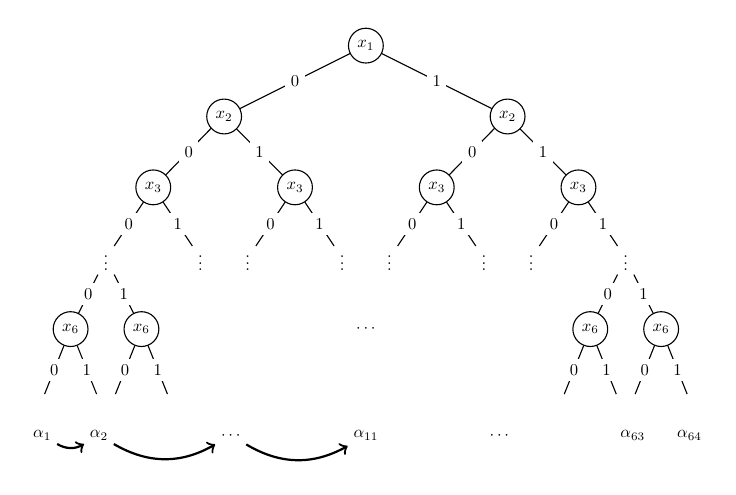
\begin{tikzpicture}[level/.style={sibling distance=60mm/#1},every node/.style={scale=0.6}, scale=0.6]
  \tikzstyle{trans}=[thick, ->, sloped]

\node [circle,draw] (x1) {$x_1$}
  child {node [circle,draw] (x2_1) {$x_2$}
    child {node [circle,draw] (x3_1) {$x_3$}
      child {node  (xn_1) {$\vdots$}
        child {node [circle,draw] (x6_1) {$x_6$}
        	child {node (x6_1f) {}
        	child[level distance=0.75cm] { node (a1) {$\alpha_1$} edge from parent[draw=none]}
        }
       		child {node (x6_1t) {}
       			child[level distance=0.75cm] { node (a2) {$\alpha_2$} edge from parent[draw=none]}
         }}
        child {node [circle,draw] (x6_2) {$x_6$}
        		child {node (x6_2f) {}}
        				child {node (x6_2t) {}
        	}
        }
      } 
      child {node (xn_2) {$\vdots$}}
    }
    child {node [circle,draw] (x3_2) {$x_3$}
      child {node (xn_3) {$\vdots$}}
      child {node (xn_4) {$\vdots$}}
    }
  }
  child {node [circle,draw] (x2_2) {$x_2$}
    child {node [circle,draw] (x3_3) {$x_3$}
      child {node (xn_5) {$\vdots$}}
      child {node (xn_6) {$\vdots$}}
    }
  child {node [circle,draw] (x3_4) {$x_3$}
    child {node (xn_7) {$\vdots$}}
    child {node (xn_8) {$\vdots$}
      child {node [circle,draw] (x6_3) {$x_6$}
      	       child {node (x6_3f) {}}
      	child {node (x6_3t) {}
        }}
      child {node [circle,draw] (x6_4) {$x_6$}
      	child {node (x6_4f) {}
        child[level distance=0.75cm] { node (an_1) {$\alpha_{63}$} edge from parent[draw=none]}
    	}
	    child {node (x6_4t) {}
    		child[level distance=0.75cm] { node (an) {$\alpha_{64}$} edge from parent[draw=none]}
      }}}
  }
};

\path (x6_2) -- (x6_3) node (x) [midway] {$\cdots$}
        child[level distance=2.25cm] { node (a_11) {$\alpha_{11}$} edge from parent[draw=none]};


\path (a2) -- (a_11) node (b1) [midway] {$\cdots$};
\path (a_11) -- (an_1) node (b2) [midway] {$\cdots$};

\draw[trans] (a1) to [bend right]  (a2);
\draw[trans] (a2) to [bend right]  (b1);
\draw[trans] (b1) to [bend right]  (a_11);

% to [bend right]  (b1) to [bend right]  (a_11);

\path (x1)   -- (x2_1) node [midway, fill=white] {$0$};
\path (x2_1) -- (x3_1) node [midway, fill=white] {$0$};
\path (x3_1) -- (xn_1) node [midway, fill=white] {$0$};
\path (xn_1) -- (x6_1) node [midway, fill=white] {$0$};
\path (x3_2) -- (xn_3) node [midway, fill=white] {$0$};
\path (x2_2) -- (x3_3) node [midway, fill=white] {$0$};
\path (x2_2) -- (x3_4) node [midway, fill=white] {$1$};
\path (x1)   -- (x2_2) node [midway, fill=white] {$1$};
\path (xn_1) -- (x6_2) node [midway, fill=white] {$1$};
\path (x3_1) -- (xn_2) node [midway, fill=white] {$1$};
\path (x2_1) -- (x3_2) node [midway, fill=white] {$1$};
\path (x3_2) -- (xn_4) node [midway, fill=white] {$1$};
\path (x3_3) -- (xn_5) node [midway, fill=white] {$0$};
\path (x3_3) -- (xn_6) node [midway, fill=white] {$1$};
\path (x3_4) -- (xn_7) node [midway, fill=white] {$0$};
\path (x3_4) -- (xn_8) node [midway, fill=white] {$1$};
\path (xn_8) -- (x6_3) node [midway, fill=white] {$0$};
\path (xn_8) -- (x6_4) node [midway, fill=white] {$1$};


\path (x6_1) -- (x6_1f) node [midway, fill=white] {$0$};
\path (x6_1) -- (x6_1t) node [midway, fill=white] {$1$};

\path (x6_2) -- (x6_2f) node [midway, fill=white] {$0$};
\path (x6_2) -- (x6_2t) node [midway, fill=white] {$1$};

\path (x6_3) -- (x6_3f) node [midway, fill=white] {$0$};
\path (x6_3) -- (x6_3t) node [midway, fill=white] {$1$};

\path (x6_4) -- (x6_4f) node [midway, fill=white] {$0$};
\path (x6_4) -- (x6_4t) node [midway, fill=white] {$1$};

\end{tikzpicture}
\end{minipage}
\begin{minipage}[c]{0.23\linewidth}
           \footnotesize
		\begin{itemize}
			\item[] $\omega_1 = \{x_1, x_2, x_3\}$ 
			\item[] $\omega_2 = \{x_4, x_5, x_6\}$
			\item[] $\omega_3 = \{\neg x_1, \neg x_5\}$
			\item[] $\omega_4 = \{\neg x_2, \neg x_4\}$
			\item[] $\omega_5 = \{\neg x_3, \neg x_4\}$
			\item[] $\omega_6 = \{\neg x_3, \neg x_6\}$
		\end{itemize}
\end{minipage}

 \caption{All possible assignments for a problem with 6 variables}
 \label{fig:naive_algo}
\end{figure}

\subsubsection{Davis Putnam Logemann Loveland algorithm (DPLL)}\label{sec:dpll}
One of the first non-memory-intensive algorithm developed to solve SAT problems is 
the Davis Putnam Logemann Loveland algorithm (DPLL)~\cite{dpll_62}. 
It explores a binary tree using depth first search as shown in \Cref{algo:dpll}.
The construction of the tree  relies on the \emph{decision} made (on \cref{algo:dpll:decision}) then,
each possible value are checked in recursive call, true value on \cref{algo:dpll:pos} and false value 
on \cref{algo:dpll:neg}.
When a leaf find a conflict (\cref{algo:dpll:unsatbranch}) which means that the formula cannot be satisfied with
the current assignment, other branches are explored.
By recursive construction of the algorithm, when each value of a literal reach to a conflict,
solver \emph{backtracks} at most one level, this fact is called \emph{chronological backtracking}.
When the conflict occurs at the top of the tree, it means that the formula cannot be satisfied and the 
solver reports $\unsat$ (\cref{algo:dpll:unsat}). However, if the formula is empty in any branch, 
it means that current assignment satisfy the whole formula and the solver reports it on \cref{algo:dpll:sat1}
or \ref{algo:dpll:sat2}.

\begin{algorithm}[!htbp]
	\SetKwProg{Fn}{function}{}{}
	\SetKwFunction{DPLL}{DPLL}	
	\SetKwFunction{unitPropagation}{unitPropagation}
	\SetKwFunction{purePropagation}{purePropagation}
	\SetKwFunction{assignDecisionLiteral}{assignDecisionLiteral}

	
	\Fn{
		\DPLL{$\varphi$: CNF formula, $\alpha$ assignment}\\
		$\quad\quad$\textbf{returns} an assignment if $\varphi$ is \sat and $\unsat$ otherwise
	}
	{	
		$\varphi, \alpha \gets$ \unitPropagation{$\varphi, \alpha$}\;
	\label{algo:dpll:unit}
		\If{$\{\} \in \varphi$}{\Return \unsat \tcp*{This branch is \unsat}}	 \label{algo:dpll:unsatbranch}
		
		\If{$\varphi = \{\}$}{\Return $\alpha$ \tcp*{$\varphi$ is $\sat$}}
		
		$x \gets$ \assignDecisionLiteral{}\; \label{algo:dpll:decision}

		\If{$\alpha \gets$ \DPLL{$\varphi \cup \{x\}, \alpha $}$\neq \unsat$ }
		{
			\Return $\alpha$ 		\label{algo:dpll:sat1}
			
		}\ElseIf{ $\alpha \gets$ \DPLL{$\varphi \cup \{\neg x\}, \alpha $}$\neq \unsat$}
		{
			\Return $\alpha$ 		\label{algo:dpll:sat2}
		} \Else{
			\Return \unsat \tcp*{$\varphi$ is $\unsat$}
		}
		\label{algo:dpll:unsat}
	}
	\caption{The DPLL algorithm.}
	\label{algo:dpll}
	
\end{algorithm}

An important function in the DPLL algorithm is \texttt{unitPropagation} (\cref{algo:dpll:unit}).
It is presented in \Cref{algo:unitdpll}. This function set value to unit clause in order to satisfy them
until fix point is reached. Either, they are no more unit clause in the formula or an inconsistency 
is found which means that current assignment cannot satisfy the formula. In the later case, the solver will
backtrack and another branch will be explored.

\begin{algorithm}
	\SetKwProg{Fn}{function}{}{}
	\SetKwFunction{unitPropagation}{unitPropagation}
	\Fn{
		\unitPropagation{$\varphi$: CNF formula, $\alpha$ assignment}\\
		$\quad\quad$\textbf{returns}  CNF formula and assignment $\alpha$ 
	}
	{	
		\While{$\{l\} \in \varphi$ \textbf{and} $\{\} \notin \varphi$  }
		{
			\tcp{\small Remove all clauses containing $l$, all literals $\neg l$}
			$\varphi \gets \varphi\mid_{\,l}$\\
			$\alpha \gets \alpha \cup \{l\}$

		}
	\Return $\varphi, \alpha$
	}
	\caption{Unit propagation}
	\label{algo:unitdpll}
	
\end{algorithm}

When DPLL algorithm is executed on the formula of \Cref{fig:naive_algo}, after making decisions on literals
$\neg x_1$ and $\neg x_2$, unit propagation detects that $x_3$ must be assigned to true.
This propagation prevents to explore  multiple assignments. Effectively, when $x_3$ is set to false value,
the clause $\omega_1$ is not satisfied and it remains 3 variables and so $2^3$ possible assignments
(from $\alpha_1$ to $\alpha_8$).
Moreover, in the DPLL algorithm, application of unit propagation until the fix point is reached leads  to a solution.
\texttt{assignDecisionLiteral} is an important procedure that responsible of choosing the variable that
divides the search space. Its objective is to find a literal that will generate a maximum of unit propagation. Intuitively, decision literals can be viewed as ‘guesses’ and propagated literals can be viewed as ‘deductions’. 
Finding a optimal variable is NP-Hard. Different heuristics exists to choose the decision variable,
some of them will be presented in the section~\ref{sec:heuristics}.

%\input{algo/puredpll}
%Another idea introduced by DPLL was \emph{elimination of pure literals},
%a literal is said pure if it only appear on one sign (positive or negative) in the problem.
%These literals are set to true in the assignment.
%On consequence, all clauses that own these literals are satisfied and so can be removed.
%
\subsubsection{Conflict Driven Clause Learning (CDCL) algorithm}\label{sec:cdcl}
The principal weakness of DPLL algorithm is to make the same inconsistencies several times
(principally due to chronological backtracking), leading to  unnecessary CPU usage.\\
Conflict Driven Clause Learning (CDCL) \cref{algo:cdcl} is a sound and complete algorithm
that overcomes principal the weakness of DPLL.

\Cref{algo:cdcl} gives an overview of CDCL, Like DPLL,  it walks on a binary search tree.
Initially, the  assignment is empty and the decision level that 
indicates the depth of the search tree, noted by $dl$, is set to zero.
The algorithm first applies unit propagation to the formula $\varphi$ for the  assignment $\alpha$ (\cref{alg:cdcl:unit}).
%Note that it is  the same procedure as the one used for DPLL.
An inconsistency or a \emph{conflict} at level zero indicates that the formula is unsatisfiable, and the algorithm
reports it (\cref{alg:cdcl:unsat_start,alg:cdcl:unsat_end}). When the conflict is occurring at a higher level, its
reason is analyzed and a clause called \emph{conflict clause} is deduced (\cref{alg:cdcl:analyze}).
The work done in this procedure will be explained thereafter.
This clause is \emph{learnt} (\cref{alg:cdcl:learn}) (added to the formula). This clause is redundant w.r.t the current
formula and so it does not change the satisfiability of $\varphi$. It also avoids encountering a conflict with the same
causes in the future.
The analysis is completed by the computation of a \emph{backjumps level} , the assignment and decision level is updated (\cref{alg:cdcl:backjump}). As the level can be much lower than the level of the current assignment, this is called \emph{non chronological backtracking}.
Finally, if no conflict appears, the algorithm chooses a new decision literal 
(\cref{alg:cdcl:pick_start,alg:cdcl:pick_end}).
The above steps are repeated until the satisfiability status of the
formula is determined.

\begin{algorithm}
	\SetKwProg{Fn}{function}{}{}
	\SetKwFunction{CDCL}{CDCL}
	\SetKwFunction{unitPropagation}{unitPropagation}
	\SetKwFunction{analyzeConflict}{analyzeConflict}
	\SetKwFunction{addLearntClause}{addLearntClause}
	\SetKwFunction{assignNewLiteral}{assignDecisionLiteral}
	\SetKwFunction{backjumpPolicy}{backjumpAndRestartPolicies}
	\SetKwFunction{ca}{currenttAssignment}
	\Fn{
		\CDCL{$\varphi$: CNF formula}\\
		$\quad\quad$\textbf{returns} $\true$ if $\varphi$ is \sat and $\false$ otherwise
	}
	{
		$dl \gets 0$ \tcp*{Current decision level}
		\While{not all variables are assigned}{
			$isConflict \gets$ \unitPropagation{}\;\label{alg:cdcl:unit}
			\If{$isConflict$}{
				\If{dl = 0}{\label{alg:cdcl:unsat_start} 
					\Return \false \label{alg:cdcl:unsat_end} 
					\tcp*{$\varphi$ is $\unsat$}
				}
				$\omega \gets$ \analyzeConflict{}\;\label{alg:cdcl:analyze} 
				$dl \gets$ \backjumpPolicy{}\;\label{alg:cdcl:backjump} 
				$\varphi \gets \varphi \cup \{\omega$\} \; \label{alg:cdcl:learn}
				
			}
			\Else{
				\assignNewLiteral{}\; \label{alg:cdcl:pick_start} 
				$dl \gets dl+1$\;\label{alg:cdcl:pick_end} 
			}
		}
		\Return \true
		\tcp*{$\varphi$ is $\sat$}
	}
	\caption{The CDCL algorithm.}
	\label{algo:cdcl}
	
\end{algorithm}

\subsection{Conflict Analysis}
A conflict is an inconsistency discovered by the solver, a situation that requires for a variable to be set 
simultaneously to the \true and \false values. \Cref{fig:conflict} shows an assignments that leads to a conflict.
First the solver choses $\neg x_1$ as a decision then, $\neg x_6$ and, then $\neg x_5$. This last one propagates $x_4$,
which in turn propagates $x_2$ and $x_3$.
To satisfy $\omega_1$, $x_3$ needs to be set to $\true$ and  to satisfy $\omega_5$, 
needs to be $\false$. As a variable cannot have both values, a conflict appears.

\begin{figure}[!htbp]
 \centering
  %{\scriptsize
%\newcommand{\ratioc}{0.195}
%\begin{minipage}[b]{\ratioc\linewidth}
%	\begin{itemize}
%		\item[] $\omega_1 = \{\cred{x_1}, x_2, x_3\}$ 
%		\item[] $\omega_2 = \{x_4, x_5, x_6\}$
%		\item[] $\cgreen{\omega_3} = \{\cgreen{\neg x_1}, \neg x_5\}$
%		\item[] $\omega_4 = \{\neg x_2, \neg x_4\}$
%		\item[] $\omega_5 = \{\neg x_3, \neg x_4\}$
%		\item[] $\omega_6 = \{\neg x_3, \neg x_6\}$
%	\end{itemize}
%\end{minipage}
%\begin{minipage}[b]{\ratioc\linewidth}
%	\begin{itemize}
%	\item[] $\omega_1 = \{\cred{x_1}, x_2, x_3\}$ 
%	\item[] $\omega_2 = \{x_4, x_5, \cred{x_6\}}$
%	\item[] $\cgreen{\omega_3} = \{\cgreen{\neg x_1}, \neg x_5\}$
%	\item[] $\omega_4 = \{\neg x_2, \neg x_4\}$
%	\item[] $\omega_5 = \{\neg x_3, \neg x_4\}$
%	\item[] $\cgreen{\omega_6} = \{\neg x_3, \cgreen{\neg x_6\}}$
%\end{itemize}
%\end{minipage}
%\begin{minipage}[b]{\ratioc\linewidth}
%		\begin{itemize}
%		\item[] $\omega_1 = \{\cred{x_1}, x_2, x_3\}$ 
%		\item[] $\omega_2 = \{\cprop{x_4}, \cred{x_5}, \cred{x_6\}}$
%		\item[] $\cgreen{\omega_3} = \{\cgreen{\neg x_1}, \cgreen{\neg x_5\}}$
%		\item[] $\omega_4 = \{\neg x_2, \neg x_4\}$
%		\item[] $\omega_5 = \{\neg x_3, \neg x_4\}$
%		\item[] $\cgreen{\omega_6} = \{\neg x_3, \cgreen{\neg x_6\}}$
%	\end{itemize}
%\end{minipage}
%\begin{minipage}[b]{\ratioc\linewidth}
%			\begin{itemize}
%		\item[] $\omega_1 = \{\cred{x_1}, x_2, x_3\}$ 
%		\item[] $\cgreen{\omega_2} = \{\cgreen{x_4}, \cred{x_5}, \cred{x_6\}}$
%		\item[] $\cgreen{\omega_3} = \{\cgreen{\neg x_1}, \cgreen{\neg x_5\}}$
%		\item[] $\omega_4 = \{\cprop{\neg x_2}, \cred{\neg x_4}\}$
%		\item[] $\omega_5 = \{\cprop{\neg x_3}, \cred{\neg x_4}\}$
%		\item[] $\cgreen{\omega_6} = \{\neg x_3, \cgreen{\neg x_6\}}$
%	\end{itemize}
%\end{minipage}
%%\begin{minipage}[b]{\ratioc\linewidth}
%%	\begin{itemize}
%%		\item[] $\omega_1 = \{\cred{x_1}, x_2, x_3\}$ 
%%		\item[] $\cgreen{\omega_2} = \{\cgreen{x_4}, \cred{x_5}, \cred{x_6\}}$
%%		\item[] $\cgreen{\omega_3} = \{\cgreen{\neg x_1}, \cgreen{\neg x_5\}}$
%%		\item[] $\omega_4 = \{\neg x_2, \cred{\neg x_4}\}$
%%		\item[] $\omega_5 = \{\neg x_3, \cred{\neg x_4}\}$
%%		\item[] $\cgreen{\omega_6} = \{\neg x_3, \cgreen{\neg x_6\}}$
%%	\end{itemize}
%%\end{minipage}
%\begin{minipage}[b]{\ratioc\linewidth}
%	\begin{itemize}
%		\item[] $\omega_1 = \{\cred{x_1}, \cred{x_2}, \cblue{x_3}\}$ 
%		\item[] $\cgreen{\omega_2} = \{\cgreen{x_4}, \cred{x_5}, \cred{x_6\}}$
%		\item[] $\cgreen{\omega_3} = \{\cgreen{\neg x_1}, \cgreen{\neg x_5\}}$
%		\item[] $\cgreen{\omega_4} = \{\cgreen{\neg x_2}, \cred{\neg x_4}\}$
%		\item[] $\omega_5 = \{\cblue{\neg x_3}, \cred{\neg x_4}\}$
%		\item[] $\cgreen{\omega_6} = \{\neg x_3, \cgreen{\neg x_6\}}$
%
%	\end{itemize}
%\end{minipage}
%}
%


\begin{tikzpicture}[level/.style={sibling distance=60mm/#1},every node/.style={scale=0.89}, scale=0.89]
	\node[text width=2.75cm] (a) {
		 $\omega_1 = \{\cred{x_1}, x_2, x_3\}$ 
		 $\omega_2 = \{x_4, x_5, x_6\}$
         $\cgreen{\omega_3} = \{\cgreen{\neg x_1}, \neg x_5\}$
	     $\omega_4 = \{\neg x_2, \neg x_4\}$
	     $\omega_5 = \{\neg x_3, \neg x_4\}$
		 $\omega_6 = \{\neg x_3, \neg x_6\}$
	};
	\node[] (al) at ($(a.south west) + (0, -0.5)$) {$\alpha$ = };
	\node[] (aa) at ($(a.south) + (0, -0.5)$) {D $\neg x_1$};
	
	\node[text width=2.75cm] (b) at ($(a) + (3.5, 0)$) {
		 $\omega_1 = \{\cred{x_1}, x_2, x_3\}$ 
		 $\omega_2 = \{x_4, x_5, \cred{x_6\}}$
		 $\cgreen{\omega_3} = \{\cgreen{\neg x_1}, \neg x_5\}$
		 $\omega_4 = \{\neg x_2, \neg x_4\}$
		 $\omega_5 = \{\neg x_3, \neg x_4\}$
		 $\cgreen{\omega_6} = \{\neg x_3, \cgreen{\neg x_6\}}$
	};
	\node[] (bb) at ($(b.south) + (0, -0.5)$) {D $\neg x_6$};
	
	\node[text width=2.75cm] (c) at ($(b) + (3.5, 0)$) {
		 $\omega_1 = \{\cred{x_1}, x_2, x_3\}$ 
		 $\omega_2 = \{\cprop{x_4}, \cred{x_5}, \cred{x_6\}}$
		 $\cgreen{\omega_3} = \{\cgreen{\neg x_1}, \cgreen{\neg x_5\}}$
		 $\omega_4 = \{\neg x_2, \neg x_4\}$
		 $\omega_5 = \{\neg x_3, \neg x_4\}$
		 $\cgreen{\omega_6} = \{\neg x_3, \cgreen{\neg x_6\}}$
	};
	\node[] (cc) at ($(c.south) + (0, -0.5)$) {D $\neg x_5$};
	
	\node[text width=2.75cm] (d) at ($(c) + (3.5, 0)$) {
		 $\omega_1 = \{\cred{x_1}, x_2, x_3\}$ 
		 $\cgreen{\omega_2} = \{\cgreen{x_4}, \cred{x_5}, \cred{x_6\}}$
		 $\cgreen{\omega_3} = \{\cgreen{\neg x_1}, \cgreen{\neg x_5\}}$
		 $\omega_4 = \{\cprop{\neg x_2}, \cred{\neg x_4}\}$
		 $\omega_5 = \{\cprop{\neg x_3}, \cred{\neg x_4}\}$
		 $\cgreen{\omega_6} = \{\neg x_3, \cgreen{\neg x_6\}}$
	};
	\node[] (dd) at ($(d.south) + (0, -0.5)$) {P $x_4$};
	
	\node[text width=2.75cm] (e) at ($(d) + (3.5, 0)$) {
		 $\omega_1 = \{\cred{x_1}, \cred{x_2}, \cblue{x_3}\}$ 
 		 $\cgreen{\omega_2} = \{\cgreen{x_4}, \cred{x_5}, \cred{x_6\}}$
 		 $\cgreen{\omega_3} = \{\cgreen{\neg x_1}, \cgreen{\neg x_5\}}$
		 $\cgreen{\omega_4} = \{\cgreen{\neg x_2}, \cred{\neg x_4}\}$
 		 $\omega_5 = \{\cblue{\neg x_3}, \cred{\neg x_4}\}$
		 $\cgreen{\omega_6} = \{\neg x_3, \cgreen{\neg x_6\}}$
	};
	\node[] (ee) at ($(e.south) + (0, -0.5)$) {P $\neg x_2$};
	\node[] (conf) at ($(e.south east) + (0, -0.5)$) {C};



	\draw[->, thick] (aa) to [bend right]  (bb);
	\draw[->, thick] (bb) to [bend right]  (cc);
	\draw[->, thick] (cc) to [bend right]  (dd);
	\draw[->, thick] (dd) to [bend right]  (ee);
	\draw[->, thick] (ee) to []  (conf);

\end{tikzpicture}

 \caption{Decisions/Propagations that leads to a  conflict}
 \label{fig:conflict}
\end{figure}
This series of decisions would provoke same propagation and leads to the same conflict. To escape this
situation, the solver needs to analyze the reason of the conflict with so-called \emph{implication graph}.
It represents the current state of the solver. It records all dependencies between  variables and  it is updated either when a variable is assigned on decision/propagation, or  when a variable
is unassigned. The implication graph is a directed acyclic graph (DAG) in which a vertex represents an assigned variable labeled by $l@dl(l)$ where $l$ represents assigned literal and $dl(l)$ represents the decision level of the literal $l$.
Root vertices , that have no incoming edges, represent decision literal. The remaining vertices represents
propagations.
Each incoming arc, labeled with a clause represents the \emph{reason} of this propagation.
This clause must be assertive, (i.e. all  literals are false except one that is not yet assigned).
\Cref{fig:implication-graph} shows the implication graph of the previous example (\Cref{fig:conflict}).
\begin{figure}[!htbp]
 \centering
 
\begin{tikzpicture} % [level/.style={sibling distance=60mm/#1},every node/.style={scale=0.89}, scale=0.89]

	\tikzstyle{decision}=[draw,double,circle,fill=red!25,minimum size=45pt,inner sep=0pt]
	\tikzstyle{propagation}=[draw,circle,fill=white!25,minimum size=45pt,inner sep=0pt]
	
	\node[decision] (dx1) {$\neg x_1$@1};
	\node[decision] (dx6) at ($(dx1) + (0, -2)$) {$\neg x_6$@2};
	\node[decision, draw=orange] (dx5) at ($(dx6) + (0, -2)$) {$\neg x_5$@3};
	
	\node[propagation, draw=orange, line width=0.5mm] (px4) at ($(dx6) + (4, -1)$) {$x_4$@3};
	\node[propagation] (px3) at ($(dx5) + (12, 0)$) {$\neg x_3$@3};
	\node[propagation] (px2) at ($(dx6) + (8, 0)$) {$\neg x_2$@3};

	\node[propagation] (px33) at ($(dx5) + (12, 4)$) {$x_3$@3};


	\node[font=\bfseries] (reason) at (2,-6) {Reason Side};
	\node[font=\bfseries] (reason) at (9,-6) {Conflict Side};

	\path[->, draw, thick] (dx6) -- (px4) node [midway, fill=white] {$\omega_2$};
	\path[->, draw, thick] (dx5) -- (px4) node [midway, fill=white] {$\omega_2$};
	
	\path[->, draw, thick] (px4) -- (px3) node [midway, fill=white] {$\omega_5$};
	\path[->, draw, thick] (px4) -- (px2) node [midway, fill=white] {$\omega_4$};
	
	\path[->, draw, thick] (dx1) -- (px33) node [midway, fill=white] {$\omega_1$};
	\path[->, draw, thick] (px2) -- (px33) node [midway, fill=white] {$\omega_1$};
7	\path[<->, draw, line width=1mm, color=blue!60] (px3) -- (px33);
	\path[line width=0.5mm, draw=orange] ($(px4.east) + (0.5, -3)$) -- ($(px4.east) + (0.5, 4)$);
	
	% Legend
	
	\path[draw] (-1, -6.5) -- (13, -6.5);
	\node[decision, scale=0.3] (ld) at (0, -7) {};
	\node[align=left, text width=2.2cm] at (1.5, -7) {Decision};
	
	\node[propagation, scale=0.3] (lp) at (0, -7.7) {};
	\node[align=left, text width=2.2cm] at (1.5, -7.7) {Propagation};
	
	\node[scale=1.5] (lz) at (5, -7) {$\rightarrow$};
	\node[align=left, text width=2.2cm] at (6.5, -7) {Implication};
	
	\node[scale=1.5] (ld) at (5, -7.7) {\textcolor{blue!60}{$\leftrightarrow$}};
	\node[align=left, text width=2.2cm] at (6.5, -7.7) {Conflict};
	
	\node[propagation, draw=orange, line width=0.5mm, scale=0.3] (le) at (10, -7) {};
	\node[align=left, text width=2.2cm] at (11.5, -7) {UIP};
	
	\node[scale=1.5] (ld) at (10, -7.7) {\textcolor{orange}{\textendash}};
	\node[align=left, text width=2.2cm] at (11.5, -7.7) {Cut};
	\path[draw] (-1, -8.2) -- (13, -8.2);
\end{tikzpicture}

 \caption{Implication graph}
 \label{fig:implication-graph}
\end{figure}

\texttt{analyzeConflict} procedure analyzes this graph to find the reason of the conflict. To do that, a search of
\emph{unique implication point} (UIP) is performed. UIP of the last decision level of the implication graph is a variable
which lies on every path from the decision to the conflict. Note that, there are many UIP for a given decision level.
In such case, UIPs are ordered according to the distance with the contradiction. The First UIP (FUIP) is the closest to
the conflict. It is well known that the first UIP provides the smallest set of assignment that is responsible for the
contradiction~\cite{zhang2001efficient}.
A UIP divides the implication graph in two sides with a \emph{cut}, the \emph{reason side} contains decision variables 
that is responsible of the contradiction and the \emph{conflict side} that contains the conflict. 
 UIP is always is the 
reason side. \Cref{fig:implication-graph} depicts two cuts in the implication graph.
Once the reason side of a conflict is established, a conflict-driven clause (or simply conflict clause) is produced.
To build this clause, it suffices to negate the
literals that have an ongoing arc to the  cut that contains the UIP. In \Cref{fig:implication-graph}, the produced
clause will be $\omega_l = \{x_1, \neg x_4 \}$. Since the information of this clause is redundant regarding 
the original formula. It can be added without any  restriction. The conflict clause can be simplified
using the implication graph to reduce its size, by detecting
redundancies~\cite{sorensson2009minimizing}. All leaned clause are store in clause database.
\texttt{backjumpAndRestartPolicies} procedure is executed after producing the conflict clause.
All responsible variables of the inconsistency are removed from the current assignment.
Adding the conflict clause prunes search space that contains no solution. This is the key point of the CDCL algorithm. In our example \Cref{fig:implication-graph}, the target decision level is 1.
After backtrack, the conflict clause will be assertive, the first UIP is the only variable that 
have not a value and will be propagated in the next step of the  algorithm.
If a conflict implies only one level, the decision variable must be assigned 
to the opposite value at level 0. This means that this literal must be true without any decision.
 
 
\subsection{Heuristics}\label{sec:heuristics}
This section gives an overview of different heuristics present in modern SAT solvers.

\textbf{Decision heuristics}. Decision variable has a huge impact on the 
overall solving time. It impacts the number of propagations and so 
the depth of the search tree.
The Variable State Independent Decaying Sum (VSIDS)~\cite{moskewicz2001chaff} measure is one of the most famous decision heuristics and is used
nowadays in almost all solvers; each variable has an activity and  is increased by a multiplicative factor 
when it participates to the resolution of a conflict.
%A solver has thousands conflicts during the solving and so activity of variables are very volatile.
Decision heuristics choose unassigned variable with the highest activity.
\hakan{AVOIR
The idea behind this heuristic is to solve ‘hard’ part of problem at the top of the search tree.
Hence, it is much more efficient when coupled with the restart heuristics}
. 
Learning rate based branching (LRB~\cite{liang2016learning}) is a latest decision heuristic. It is a
generalization of VSIDS and its goal is to optimize the \emph{learning rate} (LR), defined as the ability to generate
learned clauses. The LRB of a variable is the weighted average (computed with \emph{exponential recency
weighted average} (ERWA))  value taken by its LR over the time. Unassigned variable with the highest LRB is chose as a decision. 

\hakan{AVOIR The idea behind this heuristics is to keep variables that used to generate learned clause in the search tree.}

\textbf{Restarts.}
Another important mechanism is \emph{restart}. Basically, the solver abandons it current assignment and so 
start from the top of the tree, while maintaining other information notably learned clauses but also scores of variables in the decision heuristic. 
It prevents the solver to get stuck in ‘hard’ (heavy tailing~\cite{gomes1997heavy} part of the search space and cannot escape due 
to backjump few levels after conflict resolution. Restart is best effort heuristics, hoping that,
with more information, a better assignment was made. Hence, in practice, SAT solvers usually restart after a
certain number of conflict. Empirically a solver with restart has a better result~\cite{huang2007effect} and is today
used in almost all state-of-the-art solvers.


\textbf{Cleaning clause database.}
Storing  all learned clauses will end up by a memory issue. So, we need to develop a apolicy to eliminate
some of them. In the literatture, different criterion exists,
 the size of the clause is one of them and is very often used by solvers. Actually, a clause is really useful when 
it participates to unit propagation. The smaller the clause, the greater its chance.
\emph{Clause activity} is another heuristic, when a clause participate to conflict analysis 
its score is increment and lower activity will be removed. The last often used criteria 
is based on Literal Block Distance (LBD). It is a measure that computes the \emph{quality} of a clause
it is based on the number of decision levels present in the clause. Clauses with high value of LBD will bes
deleted from the clause database.


\subsection{Preprocessing / Inprocessing}
In order to optimize solving time, some transformation can be applied to simplify the original formula.
This is done by a \emph{preprocessing} engine before the start of solving.
When it is used during the solving, (usually after a restart), it is called \emph{inprocessing}.
Simplification of the formula is made by removing clauses and/or variables.\\

\emph{Variable elimination} simplification is based on \emph{resolution inference rule}.
Consider two clauses $\omega_1 = \{x_1, x_i, ..., x_j \}$ and $\omega_2 = \{\neg x_1, y_i, ..., y_j\}$.
The resolution inference rule allows to derive a clause $\omega_3 = \{x_i, ..., x_j, y_i, ..., y_j\}$ which is called
the \emph{resolvent} as it results from solving two clauses on the literal $x_1$ and $\neg x_1$.

Moreover,  applying variable elimination until either an empty clause is derived (unsatisfiable formula) or 
no more application of the resolution are possible (satisfiable formula). This is a complete algorithm to solve a SAT problem.
Its major issue is to explicitly generate all resolvent and can be exponential in CNF size.
Hence, the memory of the computer will be limiting factor.

\emph{The subsumption} aims at removing  clauses. Consider two clauses $\omega_1$ and $\omega_2$, such that
$\omega_1 \subset  \omega_2$, then $\omega_2$ can be safely removed from the original formula.
\emph{Self subsuming resolution} is a principle that uses resolution rules and subsumption.
The resolvent clause subsumes the original one. For example, $\omega_1 = \{x_1, \neg x_2, x_3\}$ and $\omega_2 = \{x_1, \neg x_2, x_3, x_4\}$,
 then the resolvent clause will be $\omega_3 = \{x_1, x_3\}$ which subsumes $\omega_2$. This principle
is implemented in \texttt{SatElite}~\cite{een2005effective} preprocessor engine and is used in almost all modern SAT solvers.
Other simplification techniques exist such that \emph{Gaussian elimination} which detects sub formula in a XOR-SAT
form and solve it in a polynomial time. Moreover, this technique can also be used as inprocessing~\cite{soos2010enhanced}. 
Some techniques exploit the structure of the original formula and add relevant clauses to speed up the resolution
time of the SAT solver. One of them use \textit{community structure} of the formula to find good clauses to add into.
A preprocessor engine doing that is  \texttt{modprep}~\cite{ansotegui2015using}.
The usage of symmetries also adds relevant clauses in the formula and will be detailed in the next chapter.

\subsection{Parallel SAT solving}
With the emergence of multi-core architectures and increasing power of computers, one way to optimize the solving
of a SAT problem is the exploitation of these cores. Actually, SAT problems are a good candidate for parallelism.
\emph{Portfolio} is a technique that launches several SAT solvers in parallel with different heuristics (decisions, restarts, ...) that 
communicates or not between them. When one of them finds a solution or finds that none exists, the overall computation is finished.
Another technique to develop a parallel SAT solver is called \emph{divide and conquer}. In this technique,
the search space is divided  dynamically. Several solvers cooperate to find a solution, 
%each of them is assigned to sub formula induced by the division. Some specific techniques like load balancing and work stealing 
is applied to avoid a solver to be idle.
A recent framework \emph{PaInleSS} (a Framework for Parallel SAT Solving) can be used to easily create a new parallel 
SAT solver with different heuristics~\cite{le2017painless}~\cite{le2019modular}. Authors of this framework win the parallel 
tracks of SAT competition \footnote{\url{http://www.satcompetition.org/}} in 2018.



%\begin{center}
%\begin{tikzpicture}
%\begin{scope}[blend group = soft light]
%\fill[red!30!white]   ( 90:1.2) circle (2);
%\fill[green!30!white] (210:1.2) circle (2);
%\fill[blue!30!white]  (330:1.2) circle (2);
%\end{scope}
%\node at ( 90:2)    {$x$};
%\node at ( 210:2)   {$y$};
%\node at ( 330:2)   {$z$};
%\node (c) {$x \land y \land z$};
%
%\node at ($ (c) + (-1.2, .7)$)   {$x \land y$};
%\node at ($ (c) + (+1.2, .7)$)   {$x \land z$};
%\node at ($ (c) + (0, -1.3)$)   {$y \land z$};
%\end{tikzpicture}
%\end{center}